\documentclass[fleqn]{article}

\usepackage{mydefs}
\usepackage{notes}
\usepackage{url}
\usepackage{graphicx}

\begin{document}
\lecture{CS5350: Machine Learning}{HW2: Linear Regression and 
Classification, Kernel Methods}{Due October 6, 2011}

\section{Written Exercises}

\bee

\i Consider the following variant of the sum-of-squared-errors objective for linear
regression:
\textsc{\begin{equation}
 E(\vec{w}) = \frac{1}{2}\sum_{n=1}^N r_n(y_n - \vec{w}^\top\vec{x}_n)^2
\label{eq:wtreg}
\end{equation}}
What we have basically done is modulate each of the error terms in 
the above summation using a variable $r_n$. Derive the expression 
for the weight vector $\vec{w}$ that minimizes $E(\vec{w})$. Also 
explain what role does $r_n$ play in Equation~\ref{eq:wtreg}?
(\textbf{10 marks})

Note: If it helps your calculations, you may want to rewrite the above 
objective in matrix notation (e.g., the standard 
linear regression objective $\sum_{n=1}^N (y_n - 
\vec{w}^\top\vec{x}_n)^2$ can be written as $(\vec{Y}-\vec{X}\vec{w})^\top 
(\vec{Y}-\vec{X}\vec{w})$).

\begin{solution}

Distribute the $r_n$ into the terms of errors:

\begin{eqnarray*}
 E(\vec{w}) & = & \frac{1}{2}\sum_{n=1}^N r_n(y_n - \vec{w}^\top\vec{x}_n)^2 \\
 & = & \frac{1}{2}\sum_{n=1}^N (\sqrt{r_n} y_n - \sqrt{r_n} \vec{w}^\top\vec{x}_n)^2 \\
& = & \frac{1}{2} (\sqrt{R} Y - \sqrt{R} X\vec{w})^T (\sqrt{R} Y - \sqrt{R} X\vec{w}) \\
\end{eqnarray*}

Substitute $\sqrt{R}X$ for $F$ and $\sqrt{R}Y$ for $G$:

\begin{eqnarray*}
 E(\vec{w}) & = & \frac{1}{2} (G - F\vec{w})^T (G - F\vec{w}) \\
\end{eqnarray*}

Then, the derivative follows as shown in class (for the now-identical equation $\frac{1}{2} (Y-X\vec{w})^T (Y-X\vec{w})$:

\begin{eqnarray*}
\nabla E(\vec{w}) & = & - F^T (G - F \vec{w}) \\
0 & = & - F^T (G - F \vec{w}) \\
\Rightarrow & = & F^T F \vec{w} = F^T G \\
\end{eqnarray*}

Now invert for our solution:

\begin{eqnarray*}
\hat{\vec{w}} & = & (F^T F)^{-1} F^T G \\
& = & ((\sqrt{R}X)^T \sqrt{R}X) (\sqrt{R}X)^T \sqrt{R}Y \\
\end{eqnarray*}

What does $r_n$ do here? Clearly it weighs on the estimator $\hat{\vec{w}}$, and since it's in root form, this is probably positive most of the time. This means something is only considered correct if it's \textit{more correct} than usual. This will make us more receptive to the general case, since we become less concerned with fitting tight error (as we are ignoring it to some extent), and more concerned with fitting the picture generally.

\end{solution}

\i (\textit{6350 only}) We have seen examples of regularizers
where we penalize large values of the weights by imposing 
some penalty on the norm (e.g., $\ell_2$ or $\ell_1$ norm) 
of the weight vector. It turns out that there is another way to 
accomplish the same effect: by adding some noise to each of input
variables.

Consider the linear regression model 
$y = \vec{w}^\top \vec{x}$ and the sum-of-squared-errors loss 
function 
\[
 E(\vec{w}) = \frac{1}{2}\sum_{n=1}^N \{y_n - \vec{w}^\top \vec{x}_n\}^2
\]
Let's assume we added Gaussian noise $\epsilon_n$ with zero mean
and variance $\sigma^2$ to each input $\vec{x}_n$ (so the input now
becomes $\vec{x}_n + \epsilon_n$). Show that, with the noisy inputs, 
minimizing the \textit{expected} loss function, i.e., $\mathbb{E}[E(\vec{w})]$ 
is equivalent to minimizing the original sum-of-squared-errors error for 
noise-free inputs \textit{with the addition of a weight decay regularization term}. 
The expectation $\mathbb{E}$ is w.r.t. the Gaussion noise distribution 
for which the following properties hold: $\mathbb{E}[\epsilon_n] = 0$ 
and $\mathbb{E}[\epsilon_m\epsilon_n] = \delta_{mn}\sigma^2$ (where 
$\delta_{mn}=1$ if $m=n$, and 0 otherwise). (\textbf{10 marks})

\i We saw that the Perceptron loss function can be written
as $L(\vec{w},b) = \sum_{n=1}^N \max\{0,-y_n(\vec{w}^\top\vec{x}_n+b)\}$. 
Using \textit{stochastic gradient descent} (SGD) on the loss function 
defined above, derive the Perceptron update rule which states that 
for a mispredicted training example $\vec{x}_n$:
\begin{eqnarray}
 \vec{w} &=& \vec{w} + y_n \vec{x}_n \nonumber \\
  b &=& b + y_n \nonumber
\end{eqnarray}
The stochastic gradient descent is just like gradient descent; the only 
difference is that, in each iteration, it computes the gradient using a 
single example (instead of using all the examples which standard gradient
descent does), updates the parameters using this gradient information 
(just like standard gradient descent), moves on to the next example and 
continues. (\textbf{5 marks})

\begin{solution}
Our basis is, straightforwardly, $\vec{w}^T\vec{x}_n + b$. We are given the update rules $\vec{w} = \vec{w} + y_n\vec{x}_n$ and $b = b + y_n$, and we begin by plugging them directly into this basis equation. This gives us:

\begin{eqnarray*}
\vec{w}^T_{new}\vec{x}_n + b_{new} & = & (\vec{w} + y_n\vec{x}_n)^T \vec{x}_n + b + y_n \\
& = & (\vec{w}^T + y_n\vec{x}^T_n)\vec{x}_n + b + y_n \\
& = & \vec{w}^T\vec{x}_n + y_n\vec{x}^T_n\vec{x}_n + b + y_n \\
& = & (\vec{w}^T\vec{x}_n + b) + y_n\vec{x}^T_n\vec{x}_n + y_n \\
\end{eqnarray*}

This, of course breaks down into two cases. In the first case, we've misclassified the positive example (\textit{i.e.}, $y_n = 1$), in which case we get $(\vec{w}^T\vec{x}_n + b) + \vec{x}^T_n\vec{x}_n + 1$, which we can trivially see is less negative than the basis $\vec{w}^T\vec{x}_n + b$. In the other case, we've misclassified a negative example (\textit{i.e.}, $y_n = -1$), in which case we get $(\vec{w}^T\vec{x}_n + b) - \vec{x}^T_n\vec{x}_n - 1$, which is trivially see is less positive than the basis. In both cases, we are iteratively correcting our error.

\end{solution}

\i The standard Perceptron algorithm makes an update when the incoming training example
is misclassified by the current weight vector. For the binary classification
case, we write this condition as $sign(\vec{w}^T\vec{x}+b) \neq y_n$ 
or equivalently $y_n(\vec{w}^T\vec{x}+b) < 0$. We know that if the training data
is linearly separable, the standard Perceptron will find \textit{some} hyperplane
that separates the two classes.

Now suppose we change the misclassification condition to $y_n(\vec{w}^T\vec{x}+b) 
<  \tau$ where $\tau$ is a positive constant. How does the hyperplane found
in this case differ from the standard Perceptron? Do you expect the 
new solution will generalize better or worse than the standard Perceptron on the 
test data? (\textbf{5 marks})

\begin{solution}
The old conditions tested only whether the desired classification $y_n$ and the observed result (\textit{e.g.}, the result of the postulated-hyperplane function) have different signs. This new $\tau$-based condition tests both whether they have different signs \textit{and} whether the observed result is $< \tau$. In other words, we will only consider an answer correct if it is \textit{especially} correct. This will probably generalize better, since we are ignoring the answers most likely to be incorrect, and instead fitting for the general model (though of course this depends on the exact value of $\tau$).
\end{solution}

\i In the class, we considered the non-separable case of SVM by penalizing
the misclassified training examples with a sum of slacks term ($\sum_n \xi_n$).
Consider a variation of this problem where we penalize the sum of \textbf{squared} 
slacks (i.e., $\sum_n \xi_n^2$). The optimization problem would be of the form:

\begin{gather}
\begin{split}
&   	\text{Minimize} \ \ f(\vec{w},b) = \frac{||\vec{w}||^2}{2} + \frac{C}{2} \sum_{n=1}^N \xi_n^2 \nonumber 
\\
&    	\text{subject to}\ \ \  y_n(\vec{w}^T\vec{x}_n + b) \geq 1 - \xi_n,\quad \xi_n \geq 0 \quad n=1,\ldots,N \nonumber
\end{split}
\end{gather}

Starting with this objective function, fist write down the primal Lagrangian. Then, 
optimize the primal Lagrangian with respect to $\vec{w}$ and $b$, plug these 
solutions back in and write the optimization problem just in terms of the dual 
(Lagrange) variables $\boldsymbol{\alpha}$. How does this compare to the dual formulation 
for the standard SVM where we had a sum of slacks term ($\sum_n \xi_n$)? (\textbf{10 marks})

\begin{solution}
The Primal Lagrangian is straightforwardly given from the objective function noted above:

\begin{gather*}
L_p(\vec{w}, b, \xi, \alpha, \beta) = \frac{||\vec{w}||^2}{2} + \frac{C}{2} \sum_{n=1}^N \xi_n^2 + \sum_{n=1}^N \alpha\{1-y_n(\vec{w}^T \vec{x}_n + b) - \xi_n\} - \sum_{n=1}^N \beta_n \xi_n \\
\text{subject to}\ \ \ \alpha_n, \beta_n \ge 0; n  = 1, \ldots, N
\end{gather*}

We begin by finding the partial derivatives of each relevant term:
\begin{eqnarray*}
\frac{\partial L_p}{\partial \vec{w}} & = & \sum_N (\alpha - \alpha y_n(\vec{w}^T \vec{x}_n + b) - \alpha \xi_n \\
& = & \sum_N \alpha y_n(\vec{w}^T \vec{x}_n + b) \\
\vec{w} & = & \sum_N \alpha y_n \vec{x}_n \\
\end{eqnarray*}
\begin{eqnarray*}
\frac{\partial L_p}{\partial b} & = & \sum_N \alpha(1-y_n(\vec{w}^T \vec{x}_n + b) - \xi_n) \\
& = & \sum_N \alpha y_n b \\
b & = & \sum_N \alpha y_n \\
\end{eqnarray*}
\begin{eqnarray*}
\frac{\partial L_p}{\partial \xi_n} & = & \frac{C}{2} \sum_N \xi_n^2 - \sum_N \alpha \xi_n - \beta \xi_n \\
& = & C \sum_N \xi_n - \sum_N \alpha - \beta \\
C \sum_N \xi_n & = & \sum_N \alpha - \beta \\
\xi_n & = & \frac{\alpha - \beta}{C} \\
\end{eqnarray*}

Then we plug them back into the Primal Lagrangian to get the Dual Lagrangian. Luckily the notes have given us most of this step already. All that remains is to isolate the parts that are different and add those to the end:
\begin{eqnarray*}
L_D(\vec{w}, b, \xi, \alpha, \beta) & = & \sum_N \alpha_n - \frac{1}{2} \sum_{m,n} \alpha_m \alpha_n y_m y_n (\vec{x}^T_m \vec{x}_n) + \sum_n (\alpha \xi - \beta \xi + \frac{C}{2} \xi^2) \\
& = & \sum_N \alpha_n - \frac{1}{2} \sum_{m,n} \alpha_m \alpha_n y_m y_n (\vec{x}^T_m \vec{x}_n) + \sum_n \alpha (\frac{\alpha + \beta}{C} - \beta \frac{\alpha + \beta}{C} + \frac{C}{2} \frac{\alpha + \beta}{C}) \\
& & \text{subject to } \sum_n \alpha_n y_n = 0, 0 \le a_n \le C; n \in [1..N]
\end{eqnarray*}

\end{solution}

\i Explain in 50 words (or less) why, intuitively, large margins are good. (\textbf{5 marks})

\begin{solution}
It is said that some margin $\gamma = \frac{1}{||\vec{w}||}$, so for a margin to be large, $||\vec{w}||$ must be pretty small (and thus its constituents $w_i \in \vec{w}$ must also be usually pretty small). Optimizing for simple weights tends to make simpler solutions, and this tends to point to good generalization.
\end{solution}

\i Why having a regularizer that prefers most of the entries of the weight
vector to be \textit{exactly} zero is the most desirable (call it the ``optimal
regularizer'')? Why is it difficult to accomplish this in practice? What 
alternative regularizers are actually used in practice? Rank them (a) in the order
of closeness to the optimal regularizer (closest first), (b) ease of optimization
(easiest first). Which of these regularizers do you like the most, and why?
(\textbf{5 marks})

\begin{solution}
Generally we want prediction to be based on as small a number of features as possible; as regularizers go, this typically means that we prefer as many weights in $\vec{w}$ to be $0$ as possible, since this leaves prediction to the few weights that are nonzero. Unfortunately, minimalization of the count of nonzero weights in regularizers is NP-hard, so this is usually not a feasible requirement. Alternatives are: norm-based regularizers,
\end{solution}

\i Consider a kernel function $k(\vec{x},\vec{z}) = \vec{x}^\top \vec{z}
+ 2(\vec{x}^\top \vec{z})^2$. As we know, each kernel has an associated 
feature mapping $\boldsymbol{\phi}$ such that $k(\vec{x},\vec{z}) 
= \boldsymbol{\phi}(\vec{x})^\top \boldsymbol{\phi}(\vec{z})$. Assume that
each example has two features (so $\vec{x} = \{x_1,x_2\}, \vec{z} = \{z_1,z_2\}$). 
Write down the feature mapping $\boldsymbol{\phi}$ associated with 
the kernel defined above. (\textbf{5 marks})

\begin{solution}

Given $k(\vec{x}, \vec{z}) = \vec{x}^T\vec{z} + 2(\vec{x}^T\vec{z})^2$ for $\vec{x} = \{x_1, x_2\}, \vec{z} = \{z_1, z_2\}$:

\begin{eqnarray*}
k(\vec{x}, \vec{z}) & = & (\vec{x}_1 \vec{z}_1 + \vec{x}_2 \vec{z}_2) + 2(\vec{x}_1 \vec{z}_1 + \vec{x}_2 \vec{z}_2)^2 \\
& = & (\vec{x}_1 \vec{z}_1 + \vec{x}_2 \vec{z}_2) + 2(\vec{x}^2_1 \vec{z}^2_1 + \vec{x}^2_2 \vec{z}^2_2 + 2 \vec{x}_1 \vec{x}_2 \vec{z}_1 \vec{z}_2) \\
& = & \vec{x}_1 \vec{z}_1 \vec{x}_2 \vec{z}_2 + 2 \vec{x}^2_1 \vec{z}^2_1 + 2 \vec{x}^2_2 \vec{z}^2_2 + 4 \vec{x}_1 \vec{x}_2 \vec{z}_1 \vec{z}_2 \\
& = & (\vec{x}_1, \vec{x}_2, \sqrt{2} \vec{x}^2_1, \sqrt{2} \vec{x}^2_2, 2 \vec{x}_1 \vec{x}_2)^T (\vec{z}_1, \vec{z}_2, \sqrt{2} \vec{z}^2_1, \sqrt{2} \vec{z}^2_2, 2 \vec{z}_1 \vec{z}_2) \\
\end{eqnarray*}
Thus:
\begin{eqnarray*}
\phi(\vec{x}) & = & (\vec{x}_1, \vec{x}_2, \sqrt{2} \vec{x}^2_1, \sqrt{2} \vec{x}^2_2, 2 \vec{x}_1 \vec{x}_2) \\
\phi(\vec{z}) & = & (\vec{z}_1, \vec{z}_2, \sqrt{2} \vec{z}^2_1, \sqrt{2} \vec{z}^2_2, 2 \vec{z}_1 \vec{z}_2) \\
\end{eqnarray*}
\end{solution}

\i The Euclidean distance between two points $\vec{x}$ and $\vec{z}$ is 
defined as  $||\vec{x}-\vec{z}||^2$. It's a linear distance
metric in the sense that it measures the shortest direct distance between
two points. It turns out that we can turn it to a \textit{nonlinear} distance metric
using kernels which may be useful if you want to measure the distance between
two points \textit{along} some nonlinear curve/surface. As we discussed 
while talking about kernel methods, so long as we can express an opertion in 
form of dot (inner) products, we can kernelized (i.e., non-linearize) it by
replacing each inner product by an inner product in a high dimensional feature
space. Using this fact, show that the Euclidean distance computation can be 
kernelized as well, given some kernel function $k$. Give the expression
of the nonlinearlized version of the distance function in terms of $k$. 
Also, can you think of an algorithm (among the ones you have already seen in the
class) where you could use this? (\textbf{5 marks})

\begin{solution}
Let the vectors $\vec{x} = \{x_1, x_2\}$ and $\vec{z} = \{z_1, z_2\}$. Then, let the kernel function $k(x, z) = \{x^Tz\}$. Then:
\begin{eqnarray*}
||\vec{x} - \vec{z}||_2 & = & \sqrt{(\vec{x} - \vec{z})^2} \\
& = & \sqrt{\vec{x}^T\vec{x} + \vec{z}^T\vec{z} - 2 (\vec{x}^T \vec{z})} \\
& = & \sqrt{k(\vec{x}, \vec{x}) + k(\vec{z}, \vec{z}) - 2 k(\vec{x}, \vec{z})} \\
\end{eqnarray*}
\end{solution}

\ene

\section{Programming Exercises}

\bee

\i Implement the standard Perceptron algorithm. Train it using
the provided training data and test it on the test data (ignore
the provided development data for this part). The provided
\texttt{run.m} script calls the Perceptron code (\texttt{perceptron.m}) 
which returns the Perceptron weight vector $\vec{w}$, the bias term 
$b$, and the accuracy on the test data. I have provided some skeleton code 
in \texttt{perceptron.m} and your job is to fill in the required 
pieces to make it work. See the comments in the code. Basically, you 
have to write code for testing the Perceptron update condition, the 
Perceptron update equations, and computing the predictions for the test 
data. Once you are done with these, you can simply call \texttt{run.m} 
which will print the accuracy on the test data. Report the accuracy on
the test data. (\textbf{10 marks})

\begin{solution}
My perceptron error is \texttt{0.11500}. I encourage you to run it with the \texttt{run.m} script.
\end{solution}

Now, consider the \textit{averaging extension} of the Perceptron. Note that
the standard Perceptron produces a sequence of weight vectors
(basically, an updated weight vector everytime the Perceptron makes a mistake).
However it only uses the final weight vector for making its predictions.
The averaging extension of Perceptron, on the other hand, makes use of all these
weight vectors by combining them in the following way:
note that in the standard Perceptron, each weight vector is ``good'' until 
the next mistake is made. Assume that the Perceptron produced $K$ distinct 
weight vectors $\vec{w}_1,\vec{w}_2,\ldots,\vec{w}_K$ during its training, 
and they were good for $c_1,c_2,\ldots, c_K$ exmaples respectively. The 
averaged Perceptron weight vector is given by $\sum_{k=1}^K c_k \vec{w}_k$ 
and the bias is given by $\sum_{k=1}^K c_k b_k$. In a sense, these updates
are like a weighted sum.

Implement the averaged Perceptron keeping the above logic in mind. Use the
provided skeleton code \texttt{averaged\_perceptron.m} (it's basically 
the same as the standard Perceptron's skeleton
code :-) ), and complete it to make it work for the averaged 
Perceptron case. Now, train the averaged version using the provided training 
data and test it on the test data (again, ignore the development data). 
The script \texttt{run.m} does all this for you once your averaged Perceptron 
implementation is complete. Report the accuracy on the test data. (\textbf{15 marks})

\begin{solution}
My averaged perceptron error is \texttt{0.176471}. I encourage you to run it with the \texttt{run.m} script.
\end{solution}

\i In this part, we will experiment using other people's software, 
so the programming aspect of this part will just be to write some 
short scripts for converting data formats. The software package we 
will use is libSVM \url{http://www.csie.ntu.edu.tw/~cjlin/libsvm/} 
(which, not surprisingly, implements support vector machines). You 
can either download and install these yourself, or you can use the 
version I have installed on CADE (in \texttt{$\sim$cs5350/bin}, the 
libSVM executables are \texttt{svm-train} and \texttt{svm-predict}.

The libSVM file format is one-example-per-line. The first column is 
the class (for binary this should be -1 or 1; for multiclass this should 
be a number 0, 1, 2, \ldots). The remaining columns have format $D:N$, where
$D$ is a feature number and $N$ is the feature value. I.e., our matlab format 
might have a row like:

\begin{center}
 \texttt{-1 0.2 1.5 -3.2 9.3 0 1.2}
\end{center}

The corresponding libSVM line would be something like:

\begin{center}
 \texttt{-1 1:0.2 2:1.5 3:-3.2 4:9.3 6:1.2}
\end{center}

Note that we could exclude feature 5 because its value was zero. The features 
must appear sorted (i.e., feature 1 followed by feature 2, and so on). Using 
the provided datasets, train the following SVMs (using just the training data): 
a linear SVM, a quadratic SVM, a cubic SVM and an RBF SVM. For each, try different 
values of C ranging in 0.25, 0.5, 1, 2, 4. For the RBF SVM, try $gamma$ values 
of 0.25, 0.5, 1, 2, 4. Plot error rates on both the development data and test 
data for the different values of $C$. How many support vectors are used for each 
model? Should this increase or decrease with $C$ (why?)? (\textbf{15 marks})
\ene

\begin{solution}
Notice in the following graphs that the number of support vectors steadily decreases for each of them. To answer the last question directly, the reason is because for large $C$ in $C \sum_N \xi_n$, the slack will dominate misclassifications, causing us (all else equal) to have a smaller number of misclassified examples. Unfortunately this also makes our margin smaller; either way, this is the explanation for the phenomenon you will see below.
\end{solution}

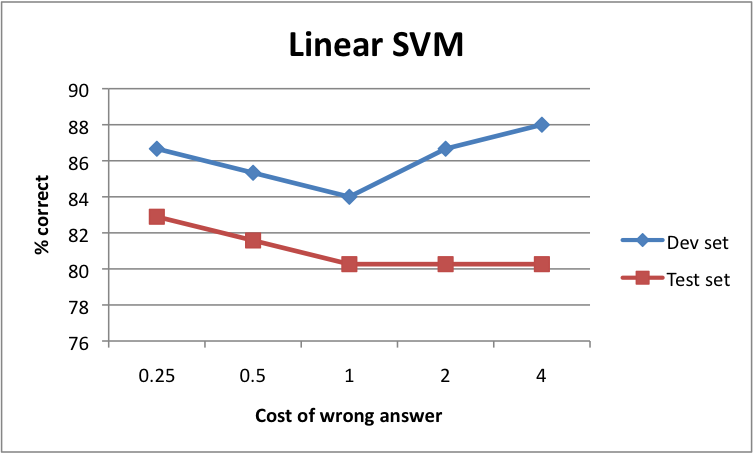
\includegraphics[scale=0.75]{linear.png} \\
The number of support vectors at each cost point for the linear SVM was, respectively: 85, 76, 73, 66, and 65. \\

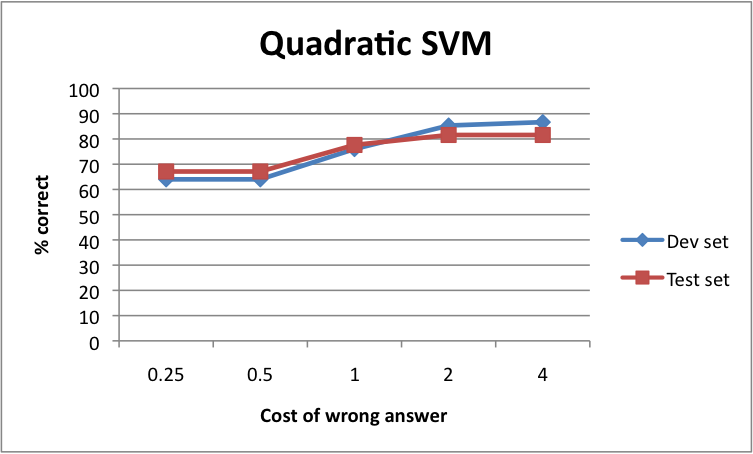
\includegraphics[scale=0.75]{quad.png} \\
The number of support vectors at each cost point for the quadratic SVM was, respectively: 155, 155, 150, 135, and 120. \\

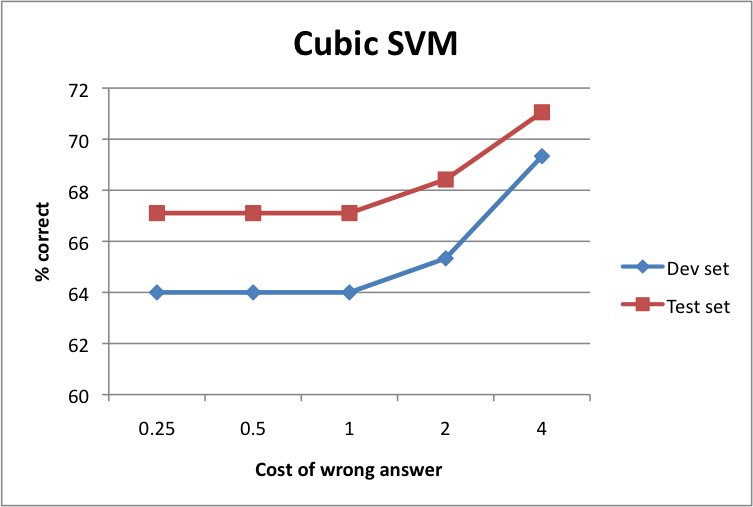
\includegraphics[scale=0.75]{cubic.png} \\
The number of support vectors at each cost point for the cubic SVM was, respectively: 152, 152, 152, 152, and 145. \\

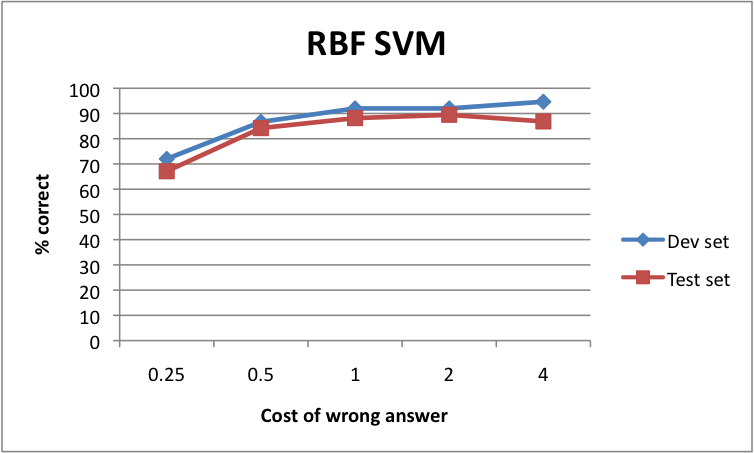
\includegraphics[scale=0.75]{rbf.png} \\
The number of support vectors at each cost point for the RBF SVM was, respectively: 144, 121, 102, 86, and81. \\

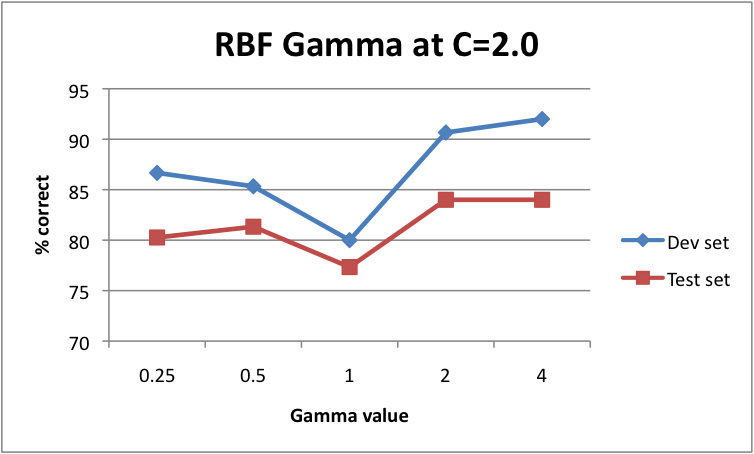
\includegraphics[scale=0.75]{gamma.png} \\
And, of course, the results of our gamma experiments follow. Rather than look at every single possible experiment, I just ran them on the best-scoring $C$. \\

\end{document}
